\documentclass{article}
\usepackage[utf8]{inputenc}
\usepackage[a4paper,top=2cm,bottom=2cm,left=3cm,right=3cm,marginparwidth=1.75cm]{geometry}
\usepackage{mathtools}
\usepackage{extarrows}
\usepackage{tcolorbox}
\usepackage{etoolbox}
\usepackage{enumitem}
\usepackage{graphicx}
\usepackage{amsmath}
\usepackage{amssymb}
\usepackage{minted}
\usepackage{float}
\usepackage{tikz}


\newtcolorbox{Codesnippet}{colback=blue!2.5!white, colframe=black!50!white}
\newtcolorbox{FullCode}{colback=black!2.5!white, colframe=black!25!white}

\renewcommand{\baselinestretch}{1.5}
\renewcommand{\contentsname}{Innholdsfortegnelse}

\graphicspath{{./images/}}

\title{REA3064: Heldagsprosjekt - Sentripitalkraft}
\author{Jonsterhaug A.V, Sørensen M.}
\date{November 2022}

\begin{document}

\maketitle

\tableofcontents
\newpage

\section{Abstrakt}
Ved hjelp av et måleapparat skal sentripetalkraften på et lodd som roterer rundt et punkt bli målt. 
Samme apparat skal brukes til å måle rotasjonen til loddet. Måledataene skal deretter bli bearbeidet 
for å regne ut vinkelfarten. Målet er å ta flere ulike måleserier med ulik masse og avstand fra sentrum på loddet, 
og se etter sammenhenger mellom vinkelfarten til loddet, og sentripetalkraften som virker på loddet.

\section{Hypotese}
Denne artikkelen ser for seg tre proporsjonaliteter i forhold til sentripitalkraften:

\begin{enumerate}
    \item En proporsjonalitet i masse
    \item En proporsjonalitet i avstanden mellom loddet og sentrum av sirkelbanen, heretter radiusen til sirkelbanen
    \item En proporsjonalitet i vinkelfart
\end{enumerate}

\noindent(1) Fra newtons lover vet man at summen av krefter på et legeme $\Sigma F = m\cdot a$ der $m$ er massen til legemet og $a$ er 
den samlede akselerasjonen på legemet. Det er derfor antatt at det eksiterer en proporsjonalitet mellom 
sentripitalkraften og massen til loddet som går i sirkelbevegelse. (2) Man har videre fra intuisjon at dersom 
loddet snurrer med større avstand, at det da vil kreve en enda større kraft for å holde den i sirkelbanen. Det er derfor intuitivt 
å tenke at det eksisterer en proporsjonalitet mellom sentripitalkraften og radiusen til sirkelbanen.
(3) Til slutt er det tenkbart at desto fortere loddet snurrer desto mer kraft kreves for å holde den i banen. 
Det er derfor antatt en sterk proporsjonalitet mellom sentripitalkraften og vinkelfarten.

\section{Matematisk utledning}
Vi skal først forsøke å utlede det matematiske uttrykket for sentripitalkraften uttrykt ved vinkelfart. Vi vet fra newtons lover at summen av 
krefter på et legeme $\Sigma F = m \cdot a$, der $m$ er legemets massen og $a$ er legemets akselerasjon. 
Ettersom at loddet her er holdt oppe av en stang som den ruller fritt over, trenger vi kun å se på kreftene som virker i det horisontale planet, 
ettersom at alle andre krefter vil nulle hverandre ut (loddet roterer i en horisontal sirkelbane som står vannrett på tyngdekraften).
De eneste kreftene som da virker på loddet er sentripitalakselerasjonen, eller mer spesifikt kraften som snoren loddet er koblet til, trekker med (se Figur 1). 
Siden massen på loddet er kjent betyr det at man kan finne en formel for sentripetalkraften ved å først finne en formel for akselerasjon. 
Dette kan oppnås ved å sette opp posisjonen til loddet som en vektorfunksjon, og deretter dobbeltderivere denne funksjonen for å finne akselerasjon, 
der $r$ er radiusen til sirkelbevegelsen, $\omega$ er vinkelfarten, $t$ er tid.
\begin{align*}
    \vec{r}(t) = [r\cos(\omega t),&\: r\sin(\omega t)]\\
    |\vec{r}(t)| =&\: r
\end{align*}

Deriverer vi posisjonsvektoren til loddet, kan vi finne et uttrykk for fartsvektoren til loddet:
\begin{align*}
    \vec{v}(t) &= \vec{r}\:'(t)\\ 
               &= [r\cos(\omega t)',\: r\sin(\omega t)']\\
               &= [-r\omega\sin(\omega t),\: r\omega\cos(\omega t)]\\
\end{align*}

Ved å derivere fartsvektoren får vi akselerasjonsvektoren som vi er ute etter:
\begin{align*}
    \vec{a}(t) &= \vec{v}\:'(t)\\ 
               &= [-r\omega^2\cos(\omega t)',\: -r\omega^2\sin(\omega t)']\\
               &= \omega^2[r\cos(\omega t),\: r\sin(\omega t)]\\
               &= \omega^2\vec{r}(t)\\
\end{align*}

Tar vi så absoluttverdien av akselerasjonsvektoren, kan vi finne et uttrykk for den rene akselerasjonen til loddet:
$$|\vec{a}(t)| = |\omega^2\vec{r}(t)|$$
$$a = \omega^2r$$

Nå som vi har en formel for akselerasjon kan vi bruke dette i utrykket for sentripetalkraften:
$$\Sigma F = m\cdot a = m\cdot \omega^2r$$

\section{Dataanalyse}
\subsection{Henting av data}
Vi har to kilder til data: en kraftmåler for å måle den faktiske sentripitalkraften, og en lysport for å finne rotasjonshastigeten til loddet.
Kraftmåleren er et analogt måleinstrument som sender ut en spenning proporsjonal med kraften som påvirker instrumentet. Lysporten består av en 
to elektriske komponenter, en diode som sender ut lys og en diode som registrerer lys, og en disk med hull i gjevne mellomrom som periodevis bryter 
lyset og slipper lyset gjennom, der antall ganger lyset blir brudt i sekundet, tilsvarer rotasjonshastigeten til apparatet. Disken er her koblet til 
loddet, og vil rotere med samme hastighet som den. Begge måleapparatene er produsert av Vernier og vi har brukt python i sammarbeid med en LabQuest 2 
for å lese av data fra måleapparatene. Python programmet har brukt Vernier sitt eget python bibliotek LabQuest for å sende dataen over USB. 
Hele programmet er vedlagt i slutten (Program 1). Målingene ble gjort over et intervall på 10 sekunder med totalt 500 målinger gjort, noe som gir en 
målefrekvens på omtrent 50 målinger i sekundet. En enda høyere målefrekvens ble ikke valgt, ettersom at det ville ført til enda større problemer med 
unøyaktigheter i måledataen, da spessielt for vinkelfarten, ettersom at dataen sendes over USB. Koden for å sette opp styringen av LabQuest-en gjennom 
python er som følger

\begin{Codesnippet}
    \begin{minted}{python}
        from labquest import LabQuest

        lq = LabQuest()
        lq.open()
        lq.select_sensors(ch1='lq_sensor', dig1='photogate_count')

        t = 10000   # Måletiden gitt i millisekunder
        n = 500     # Antall målinger

        lq.start(t/n)   # Perioden mellom målinger i millisekunder
        dig1_header = lq.enabled_sensor_info('dig1')
    \end{minted}
\end{Codesnippet}

Her velger vi å lese av et analogt signal fra kraftmåleren gjennom chanel1 og det digitale signalet fra lysporten gjennom digital1,
og starter så dataavlesningen på LabQuest-en med tidsintervallet og antall målinger som vi har spesifisert. Koden kjører så gjennom en 
løkke der den leser av dataen fra både lysporten og kraftmåleren.

\begin{Codesnippet}
    \begin{minted}{python}
        for x in range(n):
            dig1_measurement = lq.read('dig1')
            ch1_measurement = lq.read('ch1')
            if dig1_measurement == None or ch1_measurement == None:
                break
            if dig1_measurement != prev_dig1_measurement:
                file.write(f'{dig1_measurement - prev_dig1_measurement} \
                    {ch1_measurement} {time.time() - start}\n')
                prev_dig1_measurement = dig1_measurement
    \end{minted}
\end{Codesnippet}

Dataene fra kraftmåleren er analoge, og blir automatisk konvertert til newton av LabQuest biblioteket, mens for lysporten er bildet noe mer 
nyansiert. De digitale dataene lysporten spytter ut er hvor mange ganger lysstrålen har blitt brutt siden starten av programmet, og dersom 
loddet har spunnet raskt nok, vil antallet i noen tilfeller hoppe med 2 eller 3 mellom hver gang vi henter ut dataen fra instrumentet. Vi har 
derfor gjort avgjørelsen at loddet kun skal spinne en vei innenfor det samme eksperimentet, slik at vinkelfarten kun er i en retning. Etter å 
lest av hvilket antall lysporten er på, skjekker vi om den er forskjellig fra den forrige avlesningen, ettersom at vi ikke ønsker å bruke 
målinger fra kraftmåleren dersom vi ikke vet hva vinkelfarten i øyeblikket var. Vi skriver så dataen med antall lysbrudd, kraftmåling og tidsintervallet 
mellom målingene til en fil for å prosseseres og analyseres.


For å hente ut vinkelfarten fra lysport-målingene bruker vi koden under for å regne ut hvor mange radianer disken har spunnet i tidsintervallet 
mellom to påfølgende målinger, der $diff$ er listen som inneholder hvor mange brytninger som tok sted mellom de to påfølgende målingene, og $t$ 
er listen som inneholder dataen om tidene målingene ble tatt på.

\begin{Codesnippet}
    \begin{minted}{python}
        holes = 10 # Antall hull i disken
        t = data[:, 2] # Liste med tidsverdier siden start av datamåling
        w = np.zeros(len(t) - 1) # Liste med vinkelfart verdier der w[i] 
                                 # er vinkelfarten i tid t[i]
        for i in range(len(t) - 1):
            dt = t[i + 1] - t[i] # Tidsdifferanse mellom de to målingene
            w[i] = (2*np.pi / holes)*diff[i] / dt
    \end{minted}
\end{Codesnippet}

For å validere om modellen som ble utledet i seksjon 3 stemmer, har vi valgt å plotte de målte, ekte kraftmålingene opp mot den estimerte kraften 
gjennom vinkelfarten vi regnet ut ovenfor.

\subsection{Dataprossesering}
Et nytt python program (Program 2) kan nå brukes til å plotte målt sentripetalkraft i rødt, 
og estimert sentripetalkraft gitt ved vinkelfart i blått. Dersom formelen fungerer som 
forventet skal disse linjene skal ligge nærme hverandre.

\subsubsection{Rådata}

\begin{center}
    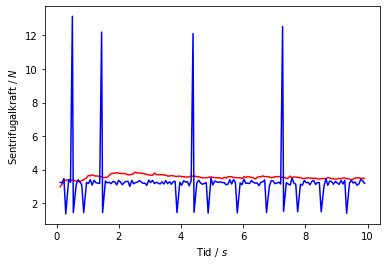
\includegraphics[width=9cm]{data_300_10.png} \\
    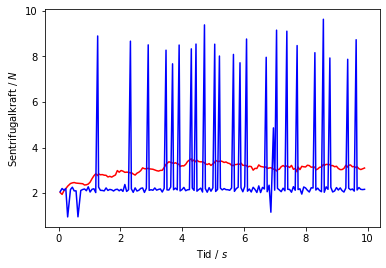
\includegraphics[width=9cm]{data_200_10.png} \\
    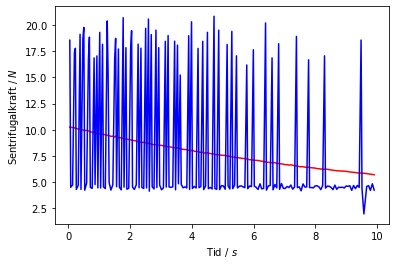
\includegraphics[width=9cm]{data_300_14.png}
\end{center}

Basert på bildene ovenfor ser det ikke ut til at den matematiske formelen fungerer særlig bra. 
Dette har sannsynligvis mye med at det bare blir gjort 50 målinger per sekund, i tillegg til at vinkelfartsmålingene 
er et gjennomsnitt av vinkelfarten over $\pi/5$ radianer, noe som kan føre til målefeil i vinkelfarten. Siden formelen 
sier at sentripetalkraften er proporsjonal med kvadratet av vinkelfarten, kan små feil i vinkelfarten føre til store feil i sentripetalkraften.

\subsubsection{Low pass filter}
For å komme oss forbi utfordingen med målefeil kan man bruke et low pass filter på målingene av vinkelfarten.
Bruker derfor en funksjon fra scipy.signal biblioteket kalt lfilter:

\begin{Codesnippet}
    \begin{minted}{python}
        scipy.signal.lfilter(b, a, x, axis=-1, zi=None)
    \end{minted}
\end{Codesnippet}

Funksjonsparameteret b er en liste med verdier mindre enn 1 slik at $\Sigma{b} = 1$, og man har da at den filtrerte verdien i en index $i$ blir 
$$\sum_{j = 0}^{w}{x\left[i + j - \frac{w}{2}\right] \cdot b[j]}$$ 
der $w$ er lengden på b og $x$ er listen med de ufiltrerte verdiene. I dette tilfellet har vi valgt at b er en liste med størrelse 20 med homogene verdier.

\begin{center}
    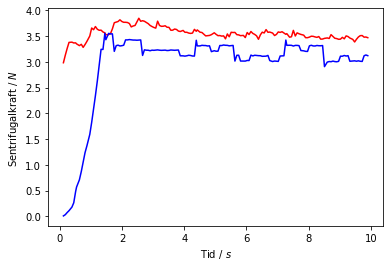
\includegraphics[width=9cm]{data_300_10_low_pass_filter.png} \\
    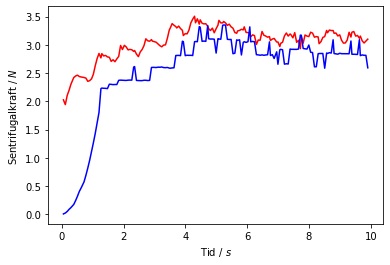
\includegraphics[width=9cm]{data_200_10_low_pass_filter.png} \\
    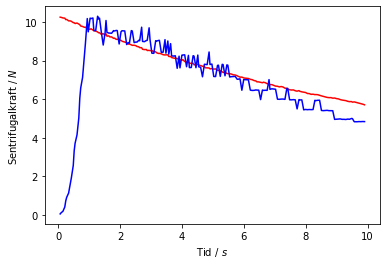
\includegraphics[width=9cm]{data_300_14_low_pass_filter.png}
\end{center}

Sannsynligvis legger funksjonen til $w$ antall 0-ere på starten og slutten av $x$, og vi ser resultatet av dette i grafen. For tidlige verdier vil funksjonen 
få langt lavere verdier enn det den skal, men etterhvert kun baserer seg på de faktiske målte verdiene for vinkelfart. Man må derfor her se bortifra tidlige verdier 
som et resultat av filtreringen, og dette er en klar nedside med denne filtreringsfunksjonen. Vi forsøkte derfor å finne en annen filtreringsfunksjon som mitigerer dette problemet.

\subsubsection{Savitzky-Golay filter}
For å unngå de dårlige startverdiene kan man bruke et Savitzky-Golay filter.

\begin{Codesnippet}
    \begin{minted}{python}
        scipy.signal.savgol_filter(x, window_length, polyorder)
    \end{minted}
\end{Codesnippet}

Funksjonen tar inn en liste med verdier $x$ som man ønsker å filtrere, $window\_length$ som er størrelsen på omegnet om en index $i$ man betrakter i filtreringen, og $polyorder$ som er 
graden til polynomet som blir brukt for å approximere inndataen.

\begin{center}
    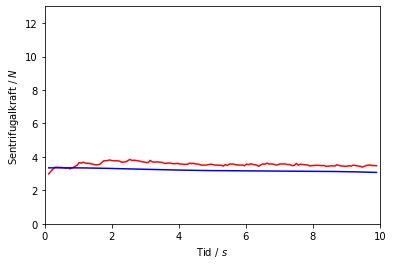
\includegraphics[width=9cm]{data_300_10_savgol_filter.png} \\
    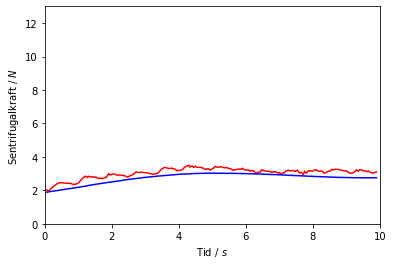
\includegraphics[width=9cm]{data_200_10_savgol_filter.png} \\
    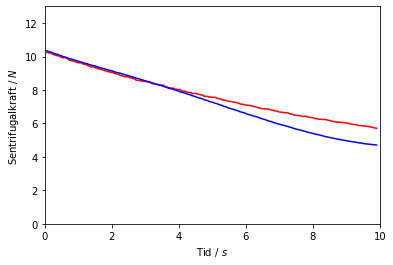
\includegraphics[width=9cm]{data_300_14_savgol_filter.png}
\end{center}

Et Savitzky-Golay filter er et digitalt filter brukt på datapunkt gjennom konvulosjon og "Linear least squares" 
for å få en utgjevnet graf som ikke mister signal tendenser i prosessen. Ved å plotte de to dataene opp mot hverandre ser 
vi at de stemmer veldig godt overens, i tillegg til at de før veldig støyete dataene for den estimerte sentripitalkraften 
nå er glatt og fin. Vi må likevel ta dataene med en klype salt, ettersom at Savitzky-Golay filteret er til dels en polynomisk 
utgjevning av inndataene.

\section{Konklusjon}
Etter å ha testet ut ulikre filtre på vinkelfarten ser det ut til at formelen $\Sigma F = m\cdot \omega^2r$ 
stemmer godt overens med målt data. Det hadde vært gunstigere å fått tak i bedre målinger for vinkelfart, 
slik at man kunne unngåt å filtrere dataene. Dette kunne blitt oppnåd ved å ta flere målinger per sekund, 
men det fungerte dårlig i praksis fordi at python programmet da ikke klarte å hente dataene like raskt 
som de ble målt.

\section{Vedlegg}

\begin{figure}[H]
    \centering
    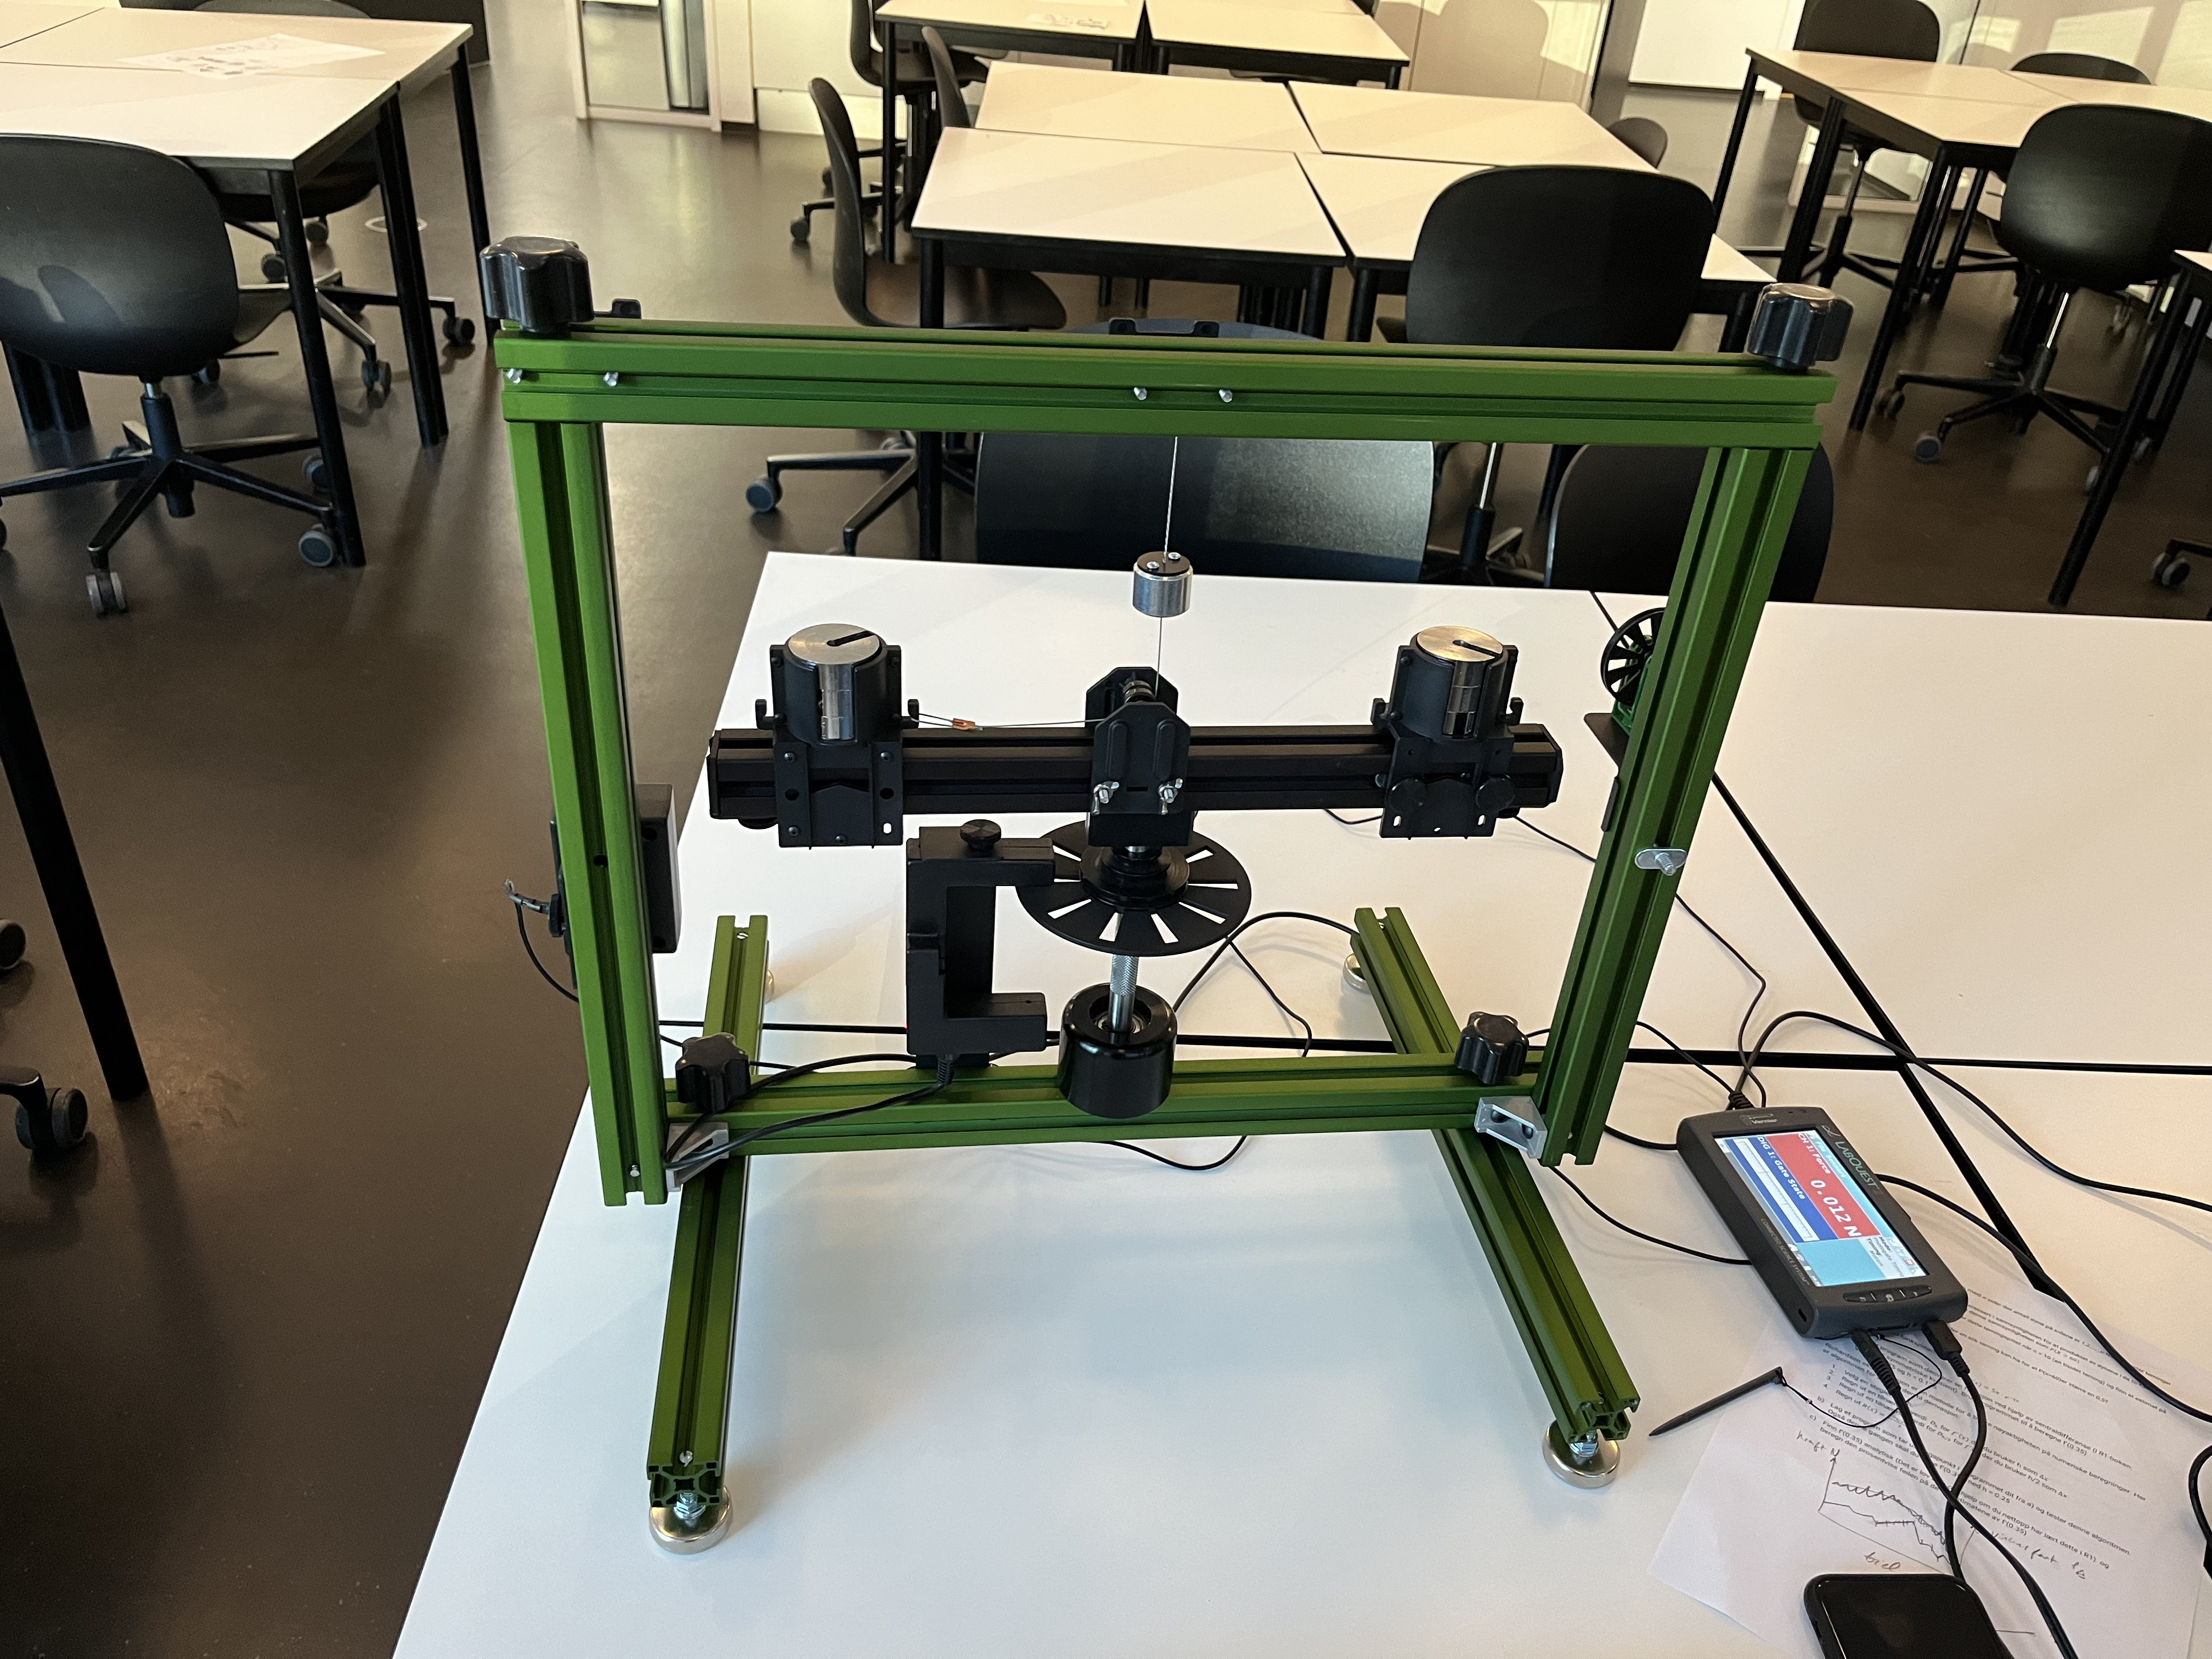
\includegraphics[width=12cm]{apparat.jpg}
    \caption{Apparat for datainnhenting}
    \label{fig:picture}
\end{figure}

\newpage
\textbf{Program 1}
\begin{FullCode}
\begin{minted}{python}
    import time
    import datetime
    from pathlib import Path
    from labquest import LabQuest

    lq = LabQuest()
    lq.open()
    lq.select_sensors(ch1='lq_sensor', dig1='photogate_count')

    t = 10000   # Måletiden gitt i millisekunder
    n = 500     # Antall målinger

    lq.start(t/n)   # Perioden mellom målinger i millisekunder
    dig1_header = lq.enabled_sensor_info('dig1')
    file = open(Path(__file__).parent / '\data_300_14.txt', 'w')
    file.write(f'Andreas V.Jonsterhaug og Morten Sørensen \
               {datetime.datetime.now()}\n\n')
    
    start = time.time()
    prev_dig1_measurement = 0

    avg = [0, 0]
    for x in range(n):
        dig1_measurement = lq.read('dig1')
        ch1_measurement = lq.read('ch1')
        if dig1_measurement == None or ch1_measurement == None:
            break
        avg[0] += ch1_measurement
        avg[1] += 1
        if dig1_measurement != prev_dig1_measurement:
            file.write(f'{dig1_measurement - prev_dig1_measurement} \
                {avg[0] / avg[1]} {time.time() - start}\n')
            prev_dig1_measurement = dig1_measurement
            avg = [0, 0]
            
    lq.stop()
    lq.close()
    file.close()
\end{minted}
\end{FullCode}

\newpage
\noindent\textbf{Program 2}
\begin{FullCode}
\begin{minted}{python}
    import matplotlib.pyplot as plt
    import numpy as np
    from scipy.signal import savgol_filter, lfilter

    d_300_10 = np.loadtxt("data_300_10.txt", skiprows=2)
    d_200_10 = np.loadtxt("data_200_10.txt", skiprows=2)
    d_300_14 = np.loadtxt("data_300_14.txt", skiprows=2)
    holes = 10

    def plot_data(diff, F, t, m, r):
        w = np.zeros(len(t) - 1)
        for i in range(len(t) - 1):
            dt = t[i + 1] - t[i]
            w[i] = (2*np.pi / holes)*diff[i] / dt

        n = len(w)
        if (n % 2 == 0): n -= 1
        w_fil = savgol_filter(w, n, 4)

        plt.xlabel("Tid / $s$")
        plt.ylabel("Sentrifugalkraft / $N$")
        ax = plt.gca()
        ax.set_xlim([0,10])
        ax.set_ylim([0,13])
        plt.plot(t[:-1], F[:-1], color="red")
        plt.plot(t[:-1], (w_fil*w_fil) * r * m, color="blue")
        plt.show()

    plot_data(d_300_10[:, 0], d_300_10[:, 1], d_300_10[:, 2], 0.3, 0.10)
    plot_data(d_200_10[:, 0], d_200_10[:, 1], d_200_10[:, 2], 0.2, 0.10)
    plot_data(d_300_14[:, 0], d_300_14[:, 1], d_300_14[:, 2], 0.3, 0.14)
\end{minted}
\end{FullCode}

\end{document}